\documentclass[sigconf]{acmart}

\AtBeginDocument{%
  \providecommand\BibTeX{{%
    Bib\TeX}}}

\definecolor{paperblue}{HTML}{7f99b0}
\newcommand{\guideline}[1]{\textit{\color{paperblue}{#1}}}
% Participant quotation: italic, set off by guillemets so the quote's own
% inner quote marks stay legible.
\newcommand{\pq}[1]{\emph{\guillemotleft #1\guillemotright}}

\paperID{UNCIRCUIT} % your project ID from your proposal

\begin{document}

\title{Exploring the Evidence and Limits of Mechanistic Explanations}

\author{Mauricio Villavicencio}
\email{mivilla@umd.edu}
\affiliation{%
 \institution{University of Maryland, College Park}
  \city{}
  \state{}
  \country{}
}

\author{Bao Ngo}
\email{baongo85@umd.edu}
\affiliation{%
 \institution{University of Maryland, College Park}
  \city{}
  \state{}
  \country{}
}

\author{Parthav Poudel}
\email{baongo85@umd.edu}
\affiliation{%
 \institution{University of Maryland, College Park}
  \city{}
  \state{}
  \country{}
}

\author{Belu Ticona}
\email{ticona.belu@gmail.com}
\affiliation{%
 \institution{George Mason University}
  \city{}
  \state{}
  \country{}
}

\begin{abstract}

\noindent Language model interfaces show how confident a model is in its answer, but not how easily that answer could be changed. Recent work measures this as the robustness margin: the smallest push to a model's internal state that changes its answer. We studied how to show this margin to people who use language models but are new to how they work inside. We built a prototype that presents the margin for 24 factual questions in four ways (a banded score, a per-layer curve, an interactive slider and a counterfactual sentence), alongside output confidence, and ran an exploratory study with 17 participants. Participants could read what each view showed and judged correctly whether the model was right in 54 of 68 predictions, but many could not explain what a margin meant or tell whether it was small. They ranked confidence as the most useful view, yet wanted the margin shown beside it. Our results suggest that a margin needs a reference point, such as a threshold suited to the task, before non-experts can make sense of it.

\noindent \textbf{Sharing preference}: This paper may be shared [publicly | with future 839E students only (default) | not at all].
\end{abstract}

\keywords{Mechanistic interpretability, uncertainty communication, interactive explanation, activation
steering, visualization design, user study}

\begin{teaserfigure}
  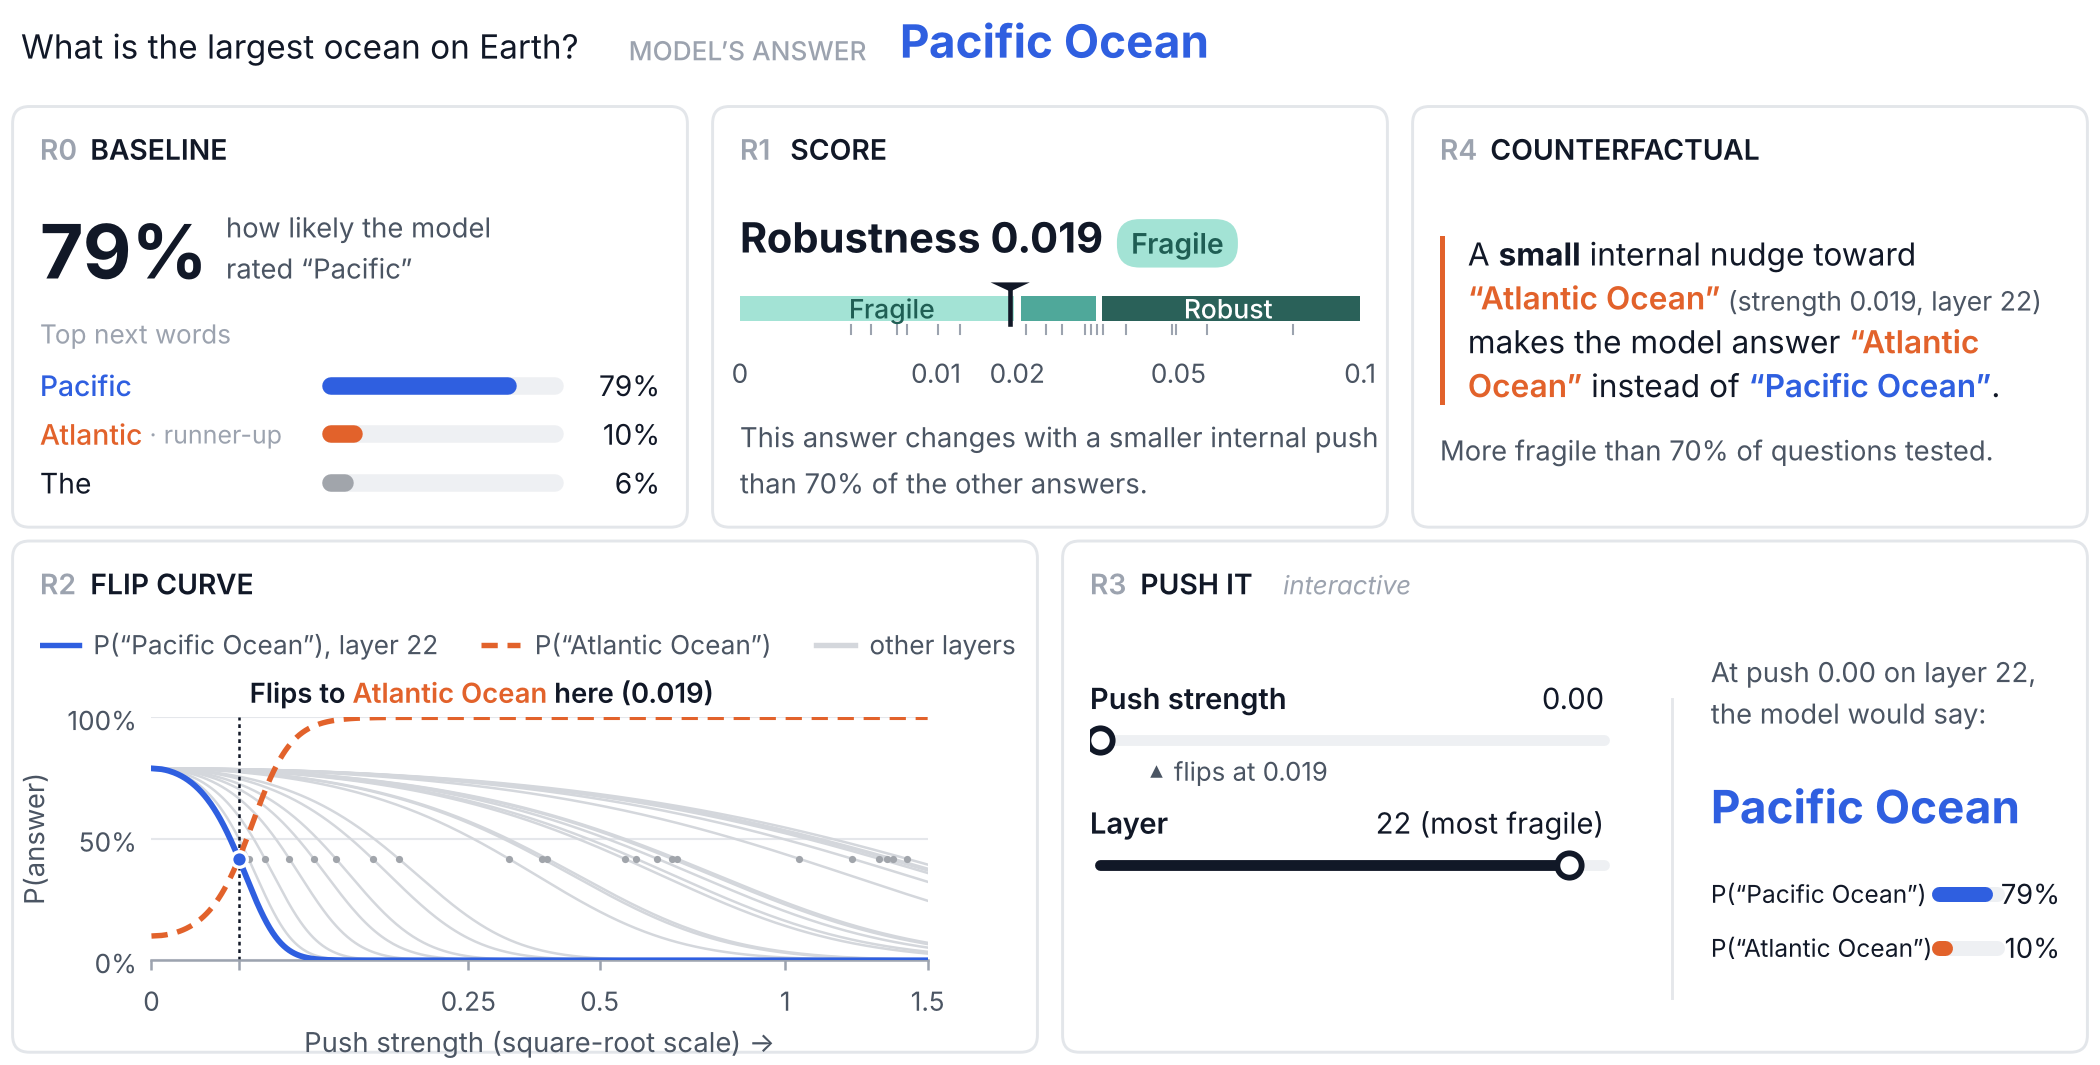
\includegraphics[width=\textwidth]{img/teaser_visual.png}
  \caption{Five views of one answer's fragility. The model answers ``Pacific Ocean'' with 79\% probability (R0), yet a push of 0.019 at layer 22 flips it to ``Atlantic Ocean'' (R1--R4).}
  \label{fig:teaser}
\end{teaserfigure}

\maketitle


\section{Introduction}

When language model interfaces report uncertainty, they usually report output confidence: the probability the
model assigns to its answer, shown as a number or put into words such as ``I'm not sure, but\ldots''
\cite{kimImNotSure2024, warrenWhenShouldTrust2026}. Confidence tells a reader how strongly the model favours its
answer. It does not tell them how much it would take to make the model give a different one.

A language model computes its answer through a stack of layers, and at each layer it holds an internal state, a
long list of numbers that carries what it has worked out so far. A small change to that state, which we call a
\emph{push}, can change the answer. \citet{komanduriMeasuringMechanisticUncertainty2026} define the
\emph{robustness margin} as the smallest push that changes the model's answer. They report that incorrect and
uncertain answers have smaller margins, and that the margin complements output-based uncertainty. The margin
could therefore tell a reader how far to trust an answer, as confidence does, but by measuring how little it
would take to change it.

How this uncertainty should be shown to people is an open question. Tools that push a model's internals help
people inspect or adjust what the model does, not judge how far to trust an answer
\cite{gevaLMDebuggerInteractiveTool2022, boSteerableChatbotsExploring2025}. Displays of fragile predictions mostly
change the input rather than the internal state \cite{dasBluffInteractivelyDeciphering2020, youPandaNotPanda2023},
and uncertainty visualization research has studied only probabilities
\cite{kayWhenIshMy2016, correllValueSuppressingUncertaintyPalettes2018}. The margin is harder to read than a
probability. Readers know that 90\% is high, but nothing tells them whether a push of 0.05 is large or small, and
the margin means little until the reader sees the different answer that push would produce.

We built a prototype\footnote{The study is at \url{https://mivillavicencio.com/interpretability_uncertainty/study/}.} that shows the robustness margin for 24 factual questions answered by
Qwen2.5-0.5B-Instruct in four forms: a banded score, a curve per layer, a slider to push the model yourself, and
a sentence describing the smallest push that changes the answer. A fifth view shows output confidence as a
baseline. Seventeen participants who use language models but are new to their internals used all five views.
We asked:

\begin{description}
  \item[RQ1] How well can non-experts read and interpret the robustness margin, and can they use it to judge
    whether a model's answer is correct?
  \item[RQ2] How do non-experts judge views of the robustness margin against output confidence?
  \item[RQ3] What design problems come up when the robustness margin is shown to non-experts?
\end{description}

We contribute a prototype that shows the robustness margin four ways alongside output confidence, an exploratory
study of how non-experts read, rank and use these views, and a set of design problems for showing the margin,
chief among them that no scale tells a reader when a margin is small. Our margin approximates the published
method, and on our questions it ranks answers much as confidence does ($\rho = 0.71$). Our findings are
therefore about how to present the margin, not about whether it adds information beyond confidence.

\section{Related Work}

Several interactive tools already let a user reach inside a model, change what it holds and watch the answer
change \cite{strobeltSeq2SeqVisVisualDebugging2018, gevaLMDebuggerInteractiveTool2022,
wangHypperSteerHypotheticalSteering2020}. This interaction is by now well established, and it is built around
a component and an expert who wants to know what that component does. A few recent systems bring it to people
who are not experts, either to teach them how a model works or to hand them a control over its behaviour
\cite{choTransformerExplainerLearning2024, boSteerableChatbotsExploring2025}. We reuse the same interaction
and give it a different purpose, which is to let a reader find out how little it takes to change an answer.

We made one of our views interactive because an explanation a reader can manipulate appears easier to grasp
than a fixed one. \citet{chengExplainingDecisionMakingAlgorithms2019} compared the two on an admissions
algorithm. The interactive version improved both how much people understood and how much they felt they
understood, where the static version improved only the first.
\citet{rossEvaluatingInterpretabilityGenerative2021a} go further and treat manipulation as a way to measure
understanding. Our tasks therefore ask participants to push the model themselves rather than only read a
display.

Work on adversarial robustness gives us the encoding for a second view, since it draws how well a prediction
holds up as a change grows stronger \cite{dasBluffInteractivelyDeciphering2020, youPandaNotPanda2023,
liVisualAnalyticsNeuron2023}. \citet{stoehrActivationScalingSteering2024} show that the strength needed to
flip a prediction is worth measuring in its own right. That is what makes a curve over push strength a
reasonable thing to draw. This work addresses practitioners who are testing a model, however, and not a reader
who is deciding whether to believe one answer.

Uncertainty visualization has studied lay readers closely, though always with probabilities rather than
margins, and two of its results shaped our design. \citet{kayWhenIshMy2016} found that readers reason better
about a chance put in concrete, countable terms than about an abstract interval.
\citet{correllValueSuppressingUncertaintyPalettes2018}, in turn, warn that a single derived number can look
more precise than the estimate behind it, which is the risk our own score runs.
\citet{fernandesUncertaintyDisplaysUsing2018} then found that the display which best helps a reader estimate a
quantity is not the one that best helps them decide with it. We therefore measured whether participants could
predict the model's answer, and not only whether they could read the numbers off the screen.

Our remaining view puts the smallest push into a sentence, following work on counterfactual explanation that
hands a user the smallest change which would alter a decision \cite{chengDECEDecisionExplorer2020,
wangGAMCoachInteractive2023}. \citet{kuhlKeepYourFriends2022} found that the nearest such change teaches a
reader more than a merely plausible one. Our sentence therefore reports the smallest push we could find rather
than a striking one.

Work on communicating a language model's own uncertainty, finally, studies the signal we use as a baseline and
has tested it as numbers, as words and as hedges \cite{kimImNotSure2024, warrenWhenShouldTrust2026,
villavicencioNotAllUncertainty2026}. \citet{boRelyNotRely2024} report that these displays reduce over-reliance
without reliably producing appropriate reliance. We read that as the bar our own views have to clear, and as a
caution against treating a preference for one view as a gain in trust.

\section{Methods}

In this study we compare four ways of showing a model's mechanistic uncertainty from the inside against a
baseline that shows ordinary output confidence. For this we rely on the definition of
\citet{komanduriMeasuringMechanisticUncertainty2026}, the smallest internal change that alters the model's
answer. Finding that change means knowing what the model would say under a given nudge, which is what a logit
lens provides. It reads a nudged internal state through the model's own output vocabulary, so for every layer
and every nudge we can see the word the model would produce instead.

We applied this method to 24 short factual questions covering world capitals, chemical elements, planets, and
notable figures in the arts and sciences, with eight questions at each of three difficulty levels. For each
question we obtain the model's preferred answer and its probability, and then, at every layer and every nudge
size, the word the model would say instead. In this way we obtained a precomputed grid over questions, layers
and nudge sizes, which is what the views we study draw on. In other words, every view shows the same numbers,
and only the way they are shown changes. We give the implementation details in Appendix~\ref{app:margin}.

The design of the views relies on three terms, which we introduce as follows. A model builds its answer over a
stack of \emph{layers}, and we can nudge the state it holds at any one of them. We call the size of a nudge its
\emph{push strength}, scaled so that it means the same thing at every layer. The \emph{margin} is the smallest
push strength that changes the answer, taken over all layers, so a small margin means the answer was easy to
change. The interface presents this margin to participants as a \emph{robustness} score, and that is the word
our questionnaire items and the quotations below use. An answer with a low score is the one we call
\emph{fragile}. We label each margin Fragile, Moderate or Robust by its rank among the 24 items. We sorted them
by margin and cut the list into three groups of eight. A band is therefore relative to this question set, and a
margin that reads as Robust here is still a small number in absolute terms. This is a simplification we adopted
to make the number legible, since no threshold marks a margin as fragile in general, and we return to it in
Section~\ref{sec:discussion}.

We chose four views that span the range of forms available, from a single number, through a chart, to direct
manipulation, to plain language. Table~\ref{tab:views} gives each one and the work it draws on.

\begin{table*}[t]
  \caption{The five views. R0 is the baseline, because output confidence is the conventional uncertainty signal
  for a language model. The other four each take a different position on how a fragility signal should reach
  a reader.}
  \label{tab:views}
  \small
  \begin{tabular}{@{}p{0.205\textwidth} p{0.405\textwidth} p{0.31\textwidth}@{}}
    \toprule
    \textbf{View} & \textbf{What it shows} & \textbf{Supporting literature} \\
    \midrule
    R0 Baseline confidence &
      The probability of the answer as a bar, with the top-5 tokens. &
      The conventional signal, and the one that work on communicating model uncertainty
      studies~\citep{kimImNotSure2024, boRelyNotRely2024}. \\
    R1 Margin score &
      The margin on a banded gauge, with a numeric label and one plain-language comparison. &
      A single summary value is the form readers take up most
      readily~\citep{kayWhenIshMy2016, correllValueSuppressingUncertaintyPalettes2018}. \\
    R2 Flip curve &
      Probability of the answer against push strength, one line per layer, with the margin layer highlighted. &
      Fragility shown as a response to perturbation
      strength~\citep{dasBluffInteractivelyDeciphering2020, youPandaNotPanda2023,
      stoehrActivationScalingSteering2024}. \\
    R3 Push it yourself &
      Sliders for strength and layer, with a live readout of what the model would answer. &
      Tools that let a user intervene on internals
      directly~\citep{gevaLMDebuggerInteractiveTool2022, wangHypperSteerHypotheticalSteering2020}. \\
    R4 Counterfactual sentence &
      One sentence naming the nudge, the target token, the strength and the layer. &
      Counterfactual explanation in plain
      language~\citep{chengDECEDecisionExplorer2020, wangGAMCoachInteractive2023, kuhlLetsGoAlien2023}. \\
    \bottomrule
  \end{tabular}
\end{table*}

\subsection{Design and procedure}

We designed the study as a self-contained web session that anyone could run on their own machine, with no
facilitator present. The interface and the questionnaire live in the same page, so participants answered each
part right after using the views rather than from memory, and the instrument recorded their responses as they
went.

We split the session into five gated parts, so that participants could not read ahead. They began
with consent and background, then explored the interface freely and reported their first impressions. Next came
guided tasks that asked them to read a view, steer the model, and predict whether its answer was right. They
then rated the five views and closed with a comprehension check and open feedback. We give the parts in full in
Appendix~\ref{app:procedure}.

Within that structure the design is within-subjects, so every participant saw all five representations, which
were also the material they were asked to rate. We counterbalanced the order of R1--R4 in the guided part,
reused that order for the ratings, and recorded it with each response. The guided tasks are graded, and we
split their items into two sets, A and B, assigned at random, so that participants working next to each other
did not converge on the same answers.

\subsection{Pilot}

Before the main study we ran a pilot round to test the interface, improve the user experience and find bugs.
We recruited about ten people, mostly classmates, and seven of them submitted complete responses. All seven
were graduate students in HCI and computer science, three at PhD level and four at master's.

Since mechanistic uncertainty is a new topic for most of our participants, what we needed to learn first was
whether people could find the controls, follow the five parts, and read what each view was showing. We did not
change the questionnaire, which is the same in the pilot and in the main study.

All six pilot participants who wrote about their first impressions reported the same problem in nearly the same
words: the interface presented everything at once and explained too little of it. One wrote that there was
\pq{a lot of information all at once, since the interface opened at `Compare All'. I wasn't sure where to start
to parse it}. Another called the interface \pq{very `in your face' with no explanations of what it does}. Four
more reported being overwhelmed by the number of graphs on the opening screen. One of them had not noticed that
the views could be opened one at a time, and another found the interface easier the longer they used it.

Based on the feedback, we realized that participants read the first impressions section as a lack of framing, a
flaw in the study rather than as part of it. That is why we made the intent visible instead of filling it in,
since explaining the two scores up front would shape the impressions we wanted to capture. We added an outline
of the study, gave free exploration its own timed part with the views hidden until the participant presses
start, and unlocked the first impressions only after three minutes.

We changed the views themselves and the guided part as well. We folded the former pop-up quick guide into two
framing steps at its start, counterbalanced exposure to R1--R4 and recorded the order, and lengthened the
view-by-view walkthrough to six to eight minutes. We also found that the views did not render consistently across
browsers, so we fixed that and checked the interface in Chrome, Safari and Firefox before the main study. The
remaining changes were minor presentation fixes, including a linear overview axis with zoom and a mini-map
after pilot participants misread the original scale, one colour per variable across the views, plainer and
larger explanations, and clearer wording in the answer key.

Because we changed the interface this much between the two rounds, we treat only the sessions run on the final
build as the main study, and every finding we report below comes from them.

\subsection{Participants}

\begin{figure}[t]
  \centering
  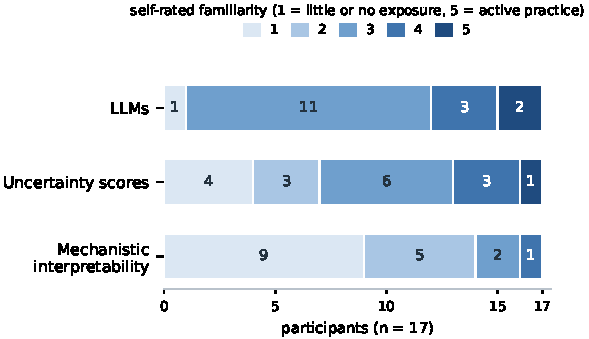
\includegraphics[width=\columnwidth]{img/familiarity.pdf}
  \caption{Self-rated familiarity of the 17 main-study participants, on a five-point scale from little or no
  exposure to active practice. Segments are counts of participants. Reading top to bottom, the medians are 3, 3
  and 1, and the means 3.29, 2.65 and 1.71.}
  \Description{Three horizontal stacked bars. Familiarity with large language models concentrates at the
  midpoint, familiarity with uncertainty scores spreads across the scale, and familiarity with mechanistic
  interpretability concentrates at the bottom.}
  \label{fig:familiarity}
\end{figure}

For the main study we recruited participants by convenience sampling, gathering them from an undergraduate NLP
class and within the authors' own network. Most were undergraduates (15 of 17, 88\%), the other two a master's
student and one who selected ``other''. Everyone took part voluntarily, remotely and at their own pace in a
browser. We did not collect any demographic information.

We asked each participant to self-rate their familiarity with large language models (LLMs), with mechanistic
interpretability and with uncertainty scores in machine learning (see Figure~\ref{fig:familiarity}). Taken
together, the three items place our participants as regular users of LLMs who are new to model internals. Each
uses a five-point scale on which 1 is little or no exposure and 5 is active practice or research. Familiarity
falls from LLMs, through uncertainty scores, to mechanistic interpretability, where 14 of 17 (82\%) sit at 1 or
2 and nobody reaches the top of the scale. When asked whether they had used a tool that edits or steers a
model's internal activations, 4 said yes, 3 said no and 10 (59\%) were not sure, more than said no.

\section{Preliminary Findings}

In the following we present our findings organized by the research questions that motivated this work.

\subsection{Reading the signal (RQ1)}

We first asked whether the choice of representation changes how accurately a non-expert reads the signal. What
we found is that participants could read the views without being able to interpret them carefully, which did not
prevent them from judging the model's answers correctly. They took values off the screen without difficulty, and
stumbled whenever a task asked what those values meant.

The graded tasks bore this out, since every participant named the word the answer flips to, and all but one read
the output confidence, the layer where the answer flips most easily, and what the answer became under a push.
The picture changed as soon as a task asked them to place a value in context rather than read it off the screen.
When we asked participants how one answer compares with the others in the set, only 9 of 17 were right, and the
rest split evenly between a wrong answer and ``not sure''.

We saw the same split in the comprehension check. Participants had no trouble saying where the push is applied
or what a small robustness score tells them. They were much less sure what a number meant, and one participant
put the gap plainly, writing that \pq{I can see what it means to be robust and fragile based on the interface,
but I wouldn't be able to describe why}.

The prediction task confirms this, since across the four items each of them considered, 54 of 68 judgements
matched whether the model's answer was right. They could put the signal to use even when they could not explain
it.

\subsection{Choosing between the views (RQ2)}

\begin{figure*}[t]
  \centering
  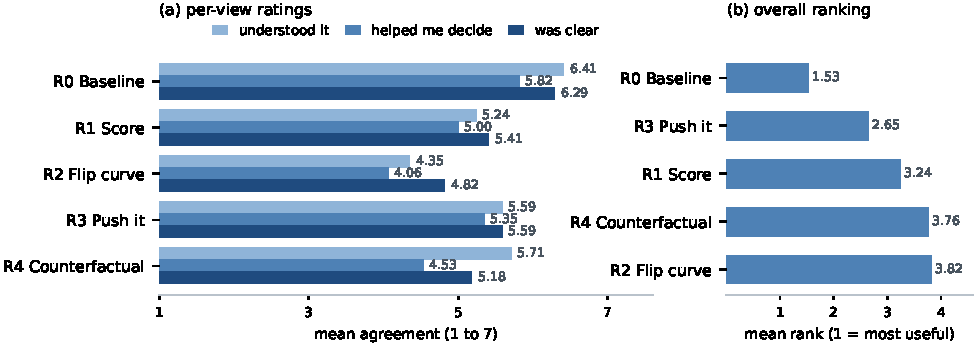
\includegraphics[width=\textwidth]{img/fig_views.pdf}
  \caption{How participants judged the five views. (a) Mean agreement with three statements about each view.
  (b) The overall ranking from most to least useful. The baseline leads on both, and the flip curve trails on
  both.}
  \Description{Grouped bars of mean agreement per view, and a bar chart of mean rank. R0 Baseline scores
  highest and ranks first. R2 Flip curve scores lowest and ranks last.}
  \label{fig:views}
\end{figure*}

We then asked which representation readers find most useful, and we observed that the baseline won. R0 took a
mean rank of 1.53, with 11 of 17 participants placing it top, while the flip curve came last at 3.82. The per-
view ratings in Figure~\ref{fig:views} point the same way, with R0 scoring highest of the five on all three
statements and R2 lowest on all three. When we asked participants which view confused them most, they named the
flip curve more often than any other, calling it \pq{crowded and hard to comprehend} and \pq{too busy}.

We noticed, however, that participants did not reject the fragility signal, a low robustness score, even though
they ranked the baseline first. They agreed that robustness told them something output confidence alone did not
(5.47 of 7), and that they would want it shown next to confidence in a model interface (5.82 of 7, median 7).
When we asked which signal they would rely on for a high-stakes question, 6 chose robustness, 6 chose both
equally, and only 3 chose output confidence. One participant concluded that \pq{while high confidence makes the
answer likely to be more true it is not set on stone and we need check robustness before trusting the answer
given}.

\subsection{Where the design broke down (RQ3)}

We asked, last, what design problems the signal surfaces when it is shown to non-experts. The clearest concern
was the scale of the metric itself, which continues the difficulty with interpretation we reported under RQ1.
When we showed participants a margin of 0.048 labelled Robust, 8 of 17 read the number as small and 5 reported
no sense of scale at all. R4 described that same strength as ``a large internal nudge'', and participants
neither agreed nor disagreed that the wording matched what they saw (4.41 of 7). One participant named the
problem directly, writing that \pq{0.048 seems small but it is labeled 91\% more internal push to change the
answer}.

We had expected a second problem that did not materialise. Letting people push the model could have made them
over-attribute control to themselves, but it did not. Instead, 13 of 17 said the slider replayed recorded
results and only one said it changed a live model. They reached that reading largely on their own, as only 6 had
noticed the caption saying the values are precomputed. Few felt they were controlling what the model would say
(3.41 of 7). Moreover, the interaction did explain stability, and watching the answer flip helped them see it
(5.94 of 7).

The session itself held together, with participants rating the interface easy to use at 6.00 of 7 and its mental
demand at 3.76 of 7. Participants again stalled on where to start, which sat at the midpoint and shows the
pilot's framing problem surviving into the main study. They also took longer than we had designed for, at a
median of 31 minutes against a 20-minute target. Overall, participants rated the study session positively, which
places the difficulty in our vocabulary rather than in the interface that carried it.

\section{Discussion and Future Work}
\label{sec:discussion}

In this study we proposed to examine how a robustness margin should be shown to someone who uses a language
model without having looked inside one. Four of our views drew on the same measurement, the smallest push
strength that changes an answer, and each put it in a different form.

Our main result is that participants recognised the relevance of robustness, the score we derived from the
margin to express mechanistic uncertainty. They used it to judge most of the model's answers correctly, and they
came to see the limits of relying on output confidence alone. They could not, however, explain the concept in
their own words, and we take recognising a signal's relevance and articulating what it measures to be different
abilities. That gap matters for trust, because someone who cannot say why an answer looks fragile has no way to
tell a sound judgement from a lucky one.

Participants showed us most clearly that the number itself carried no scale they could use. They read a value
labelled Robust and still described it as small, and several reported no sense of scale at all. We attribute
this less to our wording than to the kind of quantity it had to describe, because a probability lets a reader
picture how often something happens while the size of an intervention offers no such picture. We tried to supply
that scale by ranking our 24 items into three bands, which made the figure legible and yet let a very small
absolute value read as Robust.

Participants preferred the familiar display, and yet they did not reject the margin for it. They ranked output
confidence first and the per-layer curve last, and they still asked for the margin to appear beside confidence
rather than in place of it. We read this as agreement with \citet{komanduriMeasuringMechanisticUncertainty2026},
who proposed the margin as a complement to output-based uncertainty rather than a replacement for it. Our
findings therefore point to future work on how the two signals could be combined, rather than to a study that
asks participants which of them they prefer.

\bibliographystyle{ACM-Reference-Format}
\bibliography{refs}

\appendix

\section{The approximated margin}
\label{app:margin}

We used \texttt{Qwen2.5-0.5B-Instruct}, which has 24 decoder layers. The model answers in a few-shot,
one-word format, and we read the first token of its answer at the last prompt position. We approximate the
margin of \citet{komanduriMeasuringMechanisticUncertainty2026} rather than reproducing it.

For an item, let $a$ be the answer token, $b$ the highest-probability alternative whose decoding differs from
$a$, and $W_U$ the unembedding matrix. We take the contrastive direction

\begin{equation}
  v = W_U[b] - W_U[a], \qquad \hat{v} = \frac{v}{\lVert v \rVert},
\end{equation}

which is the Jacobian lens of \citet{komanduriMeasuringMechanisticUncertainty2026} under $J = I$. At decoder
layer $\ell$ with hidden state $h_\ell$, and at the last prompt position only, we add

\begin{equation}
  h_\ell \leftarrow h_\ell + \alpha \lVert h_\ell \rVert \hat{v},
\end{equation}

so that scaling by the residual norm leaves $\alpha$ unitless and comparable across layers. We sweep 40 values
of $\alpha$ up to $1.5$ at every layer, recording the probability of $a$, the probability of $b$ and the
current top-1 token. The per-layer margin is the smallest $\alpha$ at which the top-1 token is no longer $a$,
refined by binary search between the bracketing grid points, and the margin of an item is the minimum over
layers. We also record the layer that achieves it and the item's percentile within the set. Tokens that are
merely a different surface form of the same answer do not count as a change.

\section{Session procedure}
\label{app:procedure}

\begin{enumerate}
  \item \textbf{Consent and background (A).} Consent, program level and the familiarity items.
  \item \textbf{Free exploration, then first impressions (B).} The views stay hidden until the participant
    presses ``Start exploring'', and the questions unlock after three minutes. They ask what the interface
    shows, what ``Robustness'' means in the participant's own words, and what first confused them.
  \item \textbf{Guided tasks (C).} Two framing steps come first, one identical for everyone and one that walks
    R1--R4 in the participant's counterbalanced order. The graded tasks then cover reading an answer, steering
    with the slider, and comparing the two signals. A prediction task follows, in which participants judge for
    four items whether the model's answer is right, before the answer key unlocks.
  \item \textbf{Steering experience (D) and per-view ratings (E).} Agreement items on the push interaction,
    then ratings and a ranking of the five views, with two further items probing how the vocabulary reads.
  \item \textbf{Understanding check (F), trust and open feedback (G, H).} Graded comprehension items, agreement
    items on trust and usefulness, and free-text feedback.
\end{enumerate}

\end{document}
